\section{Filesystems}
\label{sec:filesystem}

File systems are used to dictate how data is stored and retrieved, while traditionally file systems were designed for single system, although the advancements in distributed systems, gave rise to distributed file systems (often referred to as network file systems) which are now widely deployed. However one important concern, is the underlying access control mechanism for such a system, and capabilities are better suited\cite{miltchev2008} for this for a variety of reasons:
\begin{itemize}
\item ACLs (Access Control Lists) would be a bottleneck for a distributed system, since it requires explicit authentication whereas a user possessing a capability can access the resource listed in the capability with the rights specified in it.
\item capabilities explicitly list privileges over a resource granted to the holder and hence naturally support the property of least privilege
\end{itemize} 
While access control using capabilities sets the theme for access control in distributed file systems, their implementations vary vastly as seen by the implementation detail of two popular distributed file systems, OrangeFS and TahoeLAFS. While discussing these we limit ourselves to the capability aspect without addressing the other fundamental pillars of distributed file systems such as sharding and redundancy mechanisms.

\subsection{ OrangeFS }
OrangeFS emerged as a development branch of Parallel Virtual File System (PVFS2) in 2007, and tries to address applications for the future, one of which is secure access control. PVSF2 was designed with focus on performance for parallel applications sharing data across many clients for which it uses the notion of an 'intelligent server' architecture. OrangeFS being branched out of PVFS2 is build entirely in C itself like the latter.
%OrangeFS introduced capability based security only in November 2014

OrangeFS is an object based file system, where each file and/or directory has two (or more) associated objects to it, corresponding to the metadata and the actual file data (can be split into multiple objects). Storage nodes in OrangeFS usually provide two services
\begin{itemize}
\item Metadata Service: which sends and receives the metadata of directories and logical files (the actual data need not be stored on this node)
\item Data Servce : which sends and receives data for objects stored on this node.
\end{itemize}

On a high level, OrangeFS uses a certificate based security consists of two main parts, Authentication and Access Control, and like all contemporary file systems provides access control by determining a user's access to an object based on the object's ownership and permissions. Traditionally, secure systems have used certificates to cryptographically assure verifiable identity information in storable blocks of data, these certificates are generally associated with a private and public key pair, of which the public is generally stored in the certificate along with other fields significant to the application in consideration. In case of OrangeFS the key fields are :
\begin{itemize}
\item Issuer Distinguished Name: to identify the entity that issued and signed this certificate
\item Subject Distinguished Name(DN): identifies the user that the certificate authorizes
\item Validity Period: the duration for which this issued certificate is valid.
\end{itemize} 

\begin{figure}[h]
\centering
%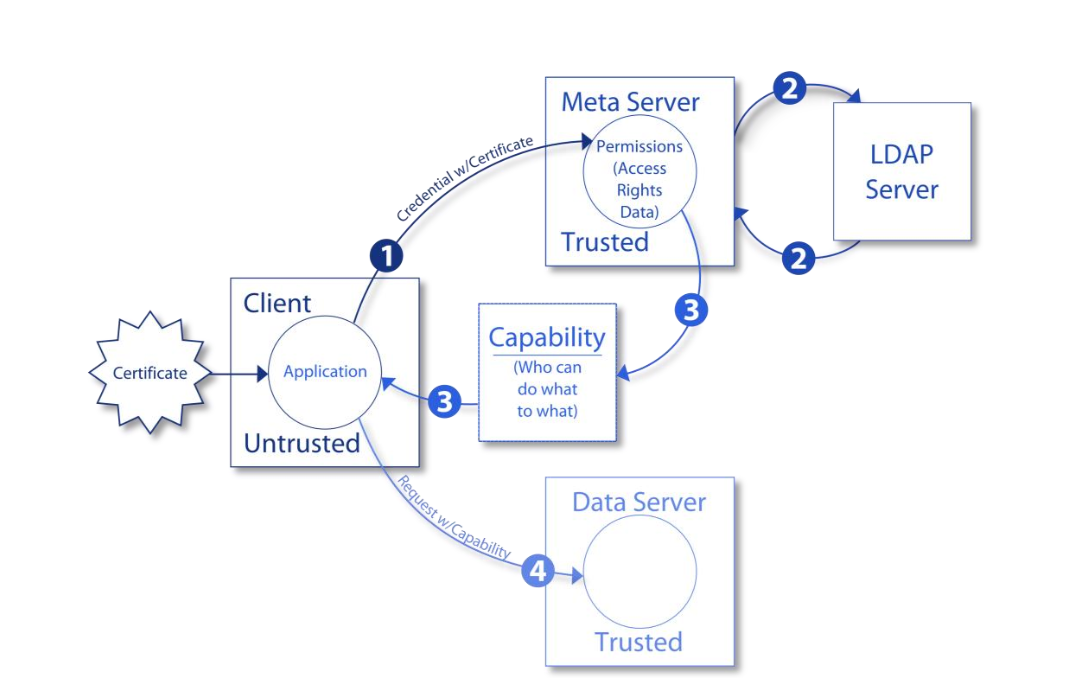
\includegraphics[scale = 0.2]{orange}
\caption{OrangeFS Architecture}
\label{fig:orange}
\end{figure}

Another entity involved in this system, is the Lightweight Directory Access Protocol(LDAP) directory which stores user objects (such as UID and GID to evaluate access rights). The Subject DN from the certificate is used to uniquely identify users in LDAP directory, and OrangeFS servers interact with LDAP servers to obtain the user information to enforce the desired access control. 

In every system that makes use of certificates for security must have a root(or roots) of trust, which can be used to issue valid certificates for other entities in the system. In OrangeFS, the trusted root certificate is called a Certificate Authority(CA) certificate, and is securely stored across each OrangeFS servers to sign and validate user certificates. Every user must have a valid user certificate (and the corresponding private key to the public key signed in their certificate) which is signed by the CA certificate. OrangeFS uses the term credential for a signed user certificate, and capabilities are signed objects containing permissions for file system objects.

As seen in Fig. \ref{fig:orange}, capability based access control can be explained in a 4 step process:
\begin{enumerate}
\item To perform a request, client sends its credential along with request to the server.
\item Server verifies credentials signature and fetches corresponding user information from the LDAP server for the subject DN in the user certificate. 
\item Server compares the user permissions with the object permissions and constructs a capability for the request.
\item Client can use the capability to act on the file system object
\end{enumerate}
One aspect to notice is that all the secure components are created with an expiration period, since revocation in a system based on capabilities can go in either two directions, by basing itself on revocation through time outs, or by using a central entity that performs revocations but there introducing a bottleneck again.

\subsection{TahoeLAFS}
One fundamental difference of TahoeLAFS(Least Authority File System) from OrangeFS is that it assures 'provider-independent security', implying that the server itself which provides the file system does not have the ability to read or modify the data, hence reducing quite a lot of latent security issues that arise from a compromised server. Moreover this bolsters their claim of true 'least-authority' semantics. This guarantee is integrated naturally into the implementation mechanism of Tahoe-LAFS and requires no additional step or management. 

TahoeLAFS\cite{tahoelafs} considers two kinds of files : mutable and immutable, and provides its access control mechanism with this in consideration. Any file uploaded to the storage grid can be chosen as either kind, and any user who has read-write access to a mutable file or directory can give other users read-write access or even any diminishing subset of the capabilities owned by the user. 

Irrespective of the type of file, all files in TahoeLAFS undergo erasure coding using Reed-Solomon codes, which allows a write to split a file into N share out which K shares need to be used to read (however Tahoe maintains small numbers for both K and N thus maintaining low computational costs for erasure coding)

\begin{figure}[h]
\centering
%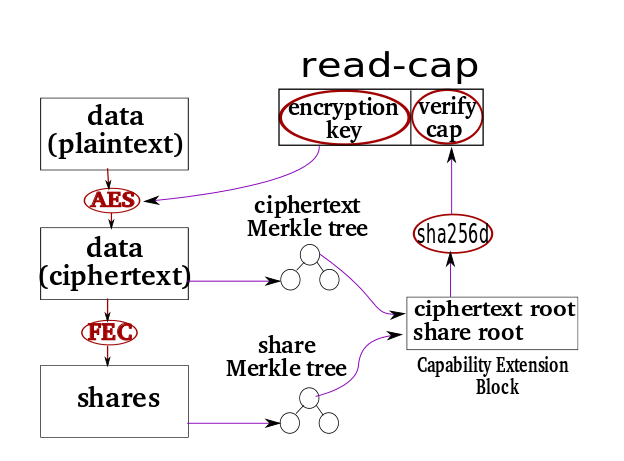
\includegraphics[scale = 0.2]{immutable}
\caption{Immutable Files in TahoeLAFS}
\label{fig:immutable}
\end{figure}

In TahoeLAFS, each immutable file has two associated capabilities, the read capability called as the \textit{read-cap} and verify capability or 
\textit{verify-cap}. To create an immutable file, the client chooses a symmetric encryption key to encrypt the file which it loads on the server. The verify-cap is derived from the ciphertext of the file using a secure hash (SHA256d\footnote{SHA256d(x) = SHA256(SHA256(x)) (to prevent length-extension attacks double SHA hashing is performed}). However verification has two problems to be taken care of
\begin{itemize}
\item If integrity check fails, client needs to isolate the erasure code shares that were wrong, for which a Merkle tree is constructed over the erasure code shares, allowing client verification of each share involved.
\item However just the Merkle Tree over erasure code shares is not sufficient as that does not link the shares to the original file content\footnote{the creator of the file could generate erasure code shares from two different files and use the shares from both in the set of N shares covered by the Merkle Tree, resulting in a different file depending on the subset of shares used to reconstruct}, and hence another Merkle Tree is constructed over the ciphertext itself.
\end{itemize}
Now, as seen in Fig.\ref{fig:immutable} the roots of both the Merkle Trees are kept on each server alongside the shares, and is called as the 'Capability Extension Block' \footnote{Logically should be part of the capability but maintained on the servers to minimize capability size}. The verify-cap is now the secure hash of the Capability Extension Block, and the read-cap to an immutable file is the verify-cap along with the original symmetric encryption key. Thus allowing the clients with the read-cap to simply pass on the verify-cap component to other clients when it wants to give it a diminished form of it's capability, moreover since the file is encrypted with the symmetric key prior to storing on to the servers, the servers themselves cannot read the data, and any attempts to modify would break the integrity check done by the verify-cap.
%footnote about choosing key can be based on the hash of plaintext of the file - convergent encryption

\begin{figure}[h]
\centering
%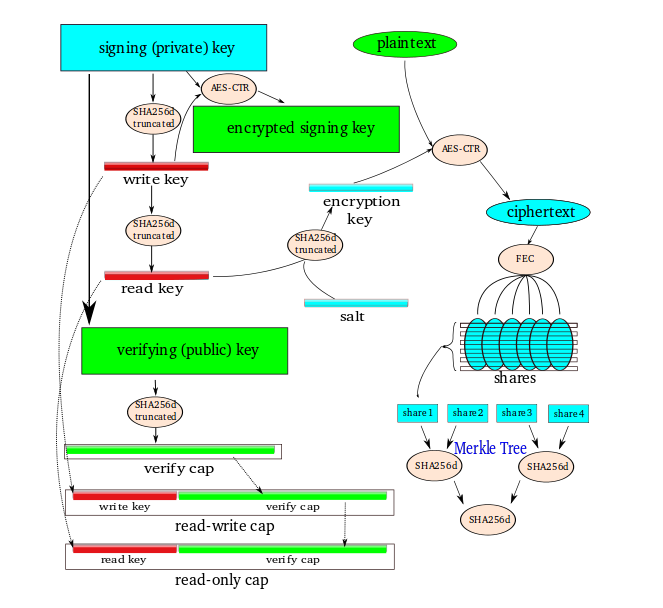
\includegraphics[scale = 0.2]{mutable}
\caption{Mutable Files in TahoeLAFS}
\label{fig:mutable}
\end{figure}

For mutable files the underlying process is significantly different and more convoluted to take care of the three desired capabilities \textit{read-write-cap}, textit{read-only-cap} and \textit{verify-cap}. Each mutable file is associated with an RSA key pair( with private key SK), a client first computes the write key, WK = SHA256d(SK) and corresponding read key, RK = SHA256d(WK). To write, a client generates a new 16 byte salt, and computes the encryption key with EK = H(RK,salt). A similar process for integrity verification is performed over the ciphertext, by computing a Merkle Tree over the erasure coded shares of the ciphertext, and the client signs the root hash of the Merkle Tree as well as the salt, with the private key SK. So the verify-cap for mutable files are the secure hash of verifying key : VC = SHA256d(VK), hence allowing clients with verify-cap to check that the verifying key which is stored on the server is the right one. The read-only cap to a mutable file include VC, and the read key RK(RC = VC,RK), while the read-write-cap to a mutable file includes VC and the write key WK (WC = VC,WK). However the owners of read-write-cap still need to be able to produce digital signatures on new versions for which the signing key SK is stored on the server encrypted with WK which is only available to the clients with read-write-cap. 

A directory could simply be treated as a mutable file which contains a set of tuples of <child name, capability to child>, this allows anyone given read access to a directory to be able to learn the child names and corresponding read capabilities, and similarly for read-write capabilities as well as for mixed capabilities for individual files of the directory. However, Tahoe implements transitive read-only access to directories, i.e. directories which have read-only access to the directory can get only a read-only-cap to a child. For this, directory includes two slots for the caps for each child, and read-write-caps for the children are encrypted separately before being stored in the mutable file.

\subsection{Comparison}
It becomes clear from the above two sections that TahoeLAFS and OrangeFS, while use the same abstraction of capability based access control mechanisms, they are entirely different in their implementation, while OrangeFS reflects a capability system with tag bits, Tahoe's implementation is based on the password/sparse capability system. Even the security properties and guarantees offered by them are different, the most significant contribution this being the notion of provider-independent security introduced in TahoeLAFS. There are many other subtle implementation details that make them highly incomparable against each other, such as the erasure coding in TahoeLAFS allows different subsections of files to be loaded from different servers, thus improving performance by improving parallelism. Moreover OrangeFS is a completely build from C, whereas TahoeLAFS is implemented in Python. Another aspect is the revocation of capabilities, while OrangeFS relies on time outs to perform revocation, in case of Tahoe since the key once given cannot be revoked, the only option is for a client to redistribute a new set of capabilities under new keys for an object, which is a significantly costly process. Hence in short, evaluating the performance of these two types of systems would not provide any insightful results.


